\section{Introducción}

Este trabajo presenta las correcciones hechas sobre el modelo de objetivos de la primer entrega. Se ha procurado incorporar más capas de negocio, y cubrir todos los requerimientos que se desprenden del enunciado original y de las sucesivas consultas a nuestro corrector (stakeholder).

\section{Lista de Requerimientos}
	\begin{description}
		\item [\namedlabel{req:R1}{R1}]. Usuario puede saber donde está el taxista.		
		\item [\namedlabel{req:R2}{R2}]. Usuario puede calificar a los taxistas.		
		\item [\namedlabel{req:R3}{R3}.] Usuario puede elegir autos y taxistas.		
		\item [\namedlabel{req:R4}{R4}.] Ofrecer viajes a los taxistas por internet.(Aviso de viaje por internet)
		\item [\namedlabel{req:R5}{R5}.] Ofrecer servicios telefónicamente.		
		\item [\namedlabel{req:R6}{R6}.] Usuarios pueden programar viajes de 
		rutina.		
		\item [\namedlabel{req:R7}{R7}.] Asistir al usuario a la elección del taxista.		
		\item [\namedlabel{req:R8}{R8}.] Directivos tienen acceso a estadísticas sobre las ganancias.
		\item [\namedlabel{req:R9}{R9}.] Directivos tienen acceso a estadísticas sobre los viajes realizados.
		\item [\namedlabel{req:R10}{R10}.] Directivos tienen acceso a estadísticas sobre las calificaciones de taxistas.
		\item [\namedlabel{req:R11}{R11}.] Envío de la información importante al sistema estadístico.
		\item [\namedlabel{req:R12}{R12}.] (Evitar) Acceso de personal no autorizado a info relevante.
		
		\item [\namedlabel{req:R14}{R14}.] Mostrar al usuario el ranking de taxistas disponibles de acuerdo al orden de calificaciones y de distancias.
		\item [\namedlabel{req:R15}{R15}.] Al mostrar taxistas siempre mostrar el taxi que maneja.
		\item [\namedlabel{req:R16}{R16}.] Historial de calificaciones de los taxistas
		\item [\namedlabel{req:R17}{R17}.] Elaboración de lista de taxistas ordenados según puntuación en las calificaciones.
		\item [\namedlabel{req:R18}{R18}.] Calcular distancias entre taxistas y usuarios.
		\item [\namedlabel{req:R19}{R19}.] Elaboración de la lista de taxistas ordenados según distancia a ubicación de usuario.
		\item [\namedlabel{req:R20}{R20}.] Mostrar menú de viajes a los usuarios logueados.
		\item [\namedlabel{req:R21}{R21}.] Ofrecer servicio del menú de viajes a los usuarios que llamen.
		\item [\namedlabel{req:R22}{R22}.] Si no hay internet, comunicar viajes a operadora.
		\item [\namedlabel{req:R23}{R23}.] Usuarios pueden calificar a los taxistas.		
		\item [\namedlabel{req:R24}{R24}.] Almacenar calificación de taxista como info importante.
		\item [\namedlabel{req:R26}{R26}.] Registro de importe cobrado.
		\item [\namedlabel{req:R27}{R27}.] Si taxista no acepta, comunicarselo al usuario.
		\item [\namedlabel{req:R28}{R28}.] Aviso por internet de viaje de rutina en fecha pactada por el usuario.
		\item [\namedlabel{req:R29}{R29}.] Si no hay internet, comunicación de viaje a operadora.
		\item [\namedlabel{req:R30}{R30}.] Usuarios pueden calificar a los taxistas.
		\item [\namedlabel{req:R31}{R31}.] Historial de calificación de taxista.
		\item [\namedlabel{req:R32}{R32}.] Comunicar a sistema de pago el monto a cobrar.
		\item [\namedlabel{req:R33}{R33}.] Calcular costo del viaje según la distancia obtenida.
		\item [\namedlabel{req:R34}{R34}.] Calcular costo del viaje según la distancia obtenida.
		\item [\namedlabel{req:R35}{R35}.] Comunicar al taxista importe del viaje.
		\item [\namedlabel{req:R36}{R36}.] Almacenar importe como información importante.
		\item [\namedlabel{req:R37}{R37}.] Usuario puede cancelar viajes que no comenzaron.
		\item [\namedlabel{req:R38}{R38}.] Comunicar al taxista de la cancelación por intenet.
		\item [\namedlabel{req:R39}{R39}.] Comunicar al taxista de cancelación por radio.

		
	\end{description}
	

\section{Diagramas del Modelo de Objetivos}
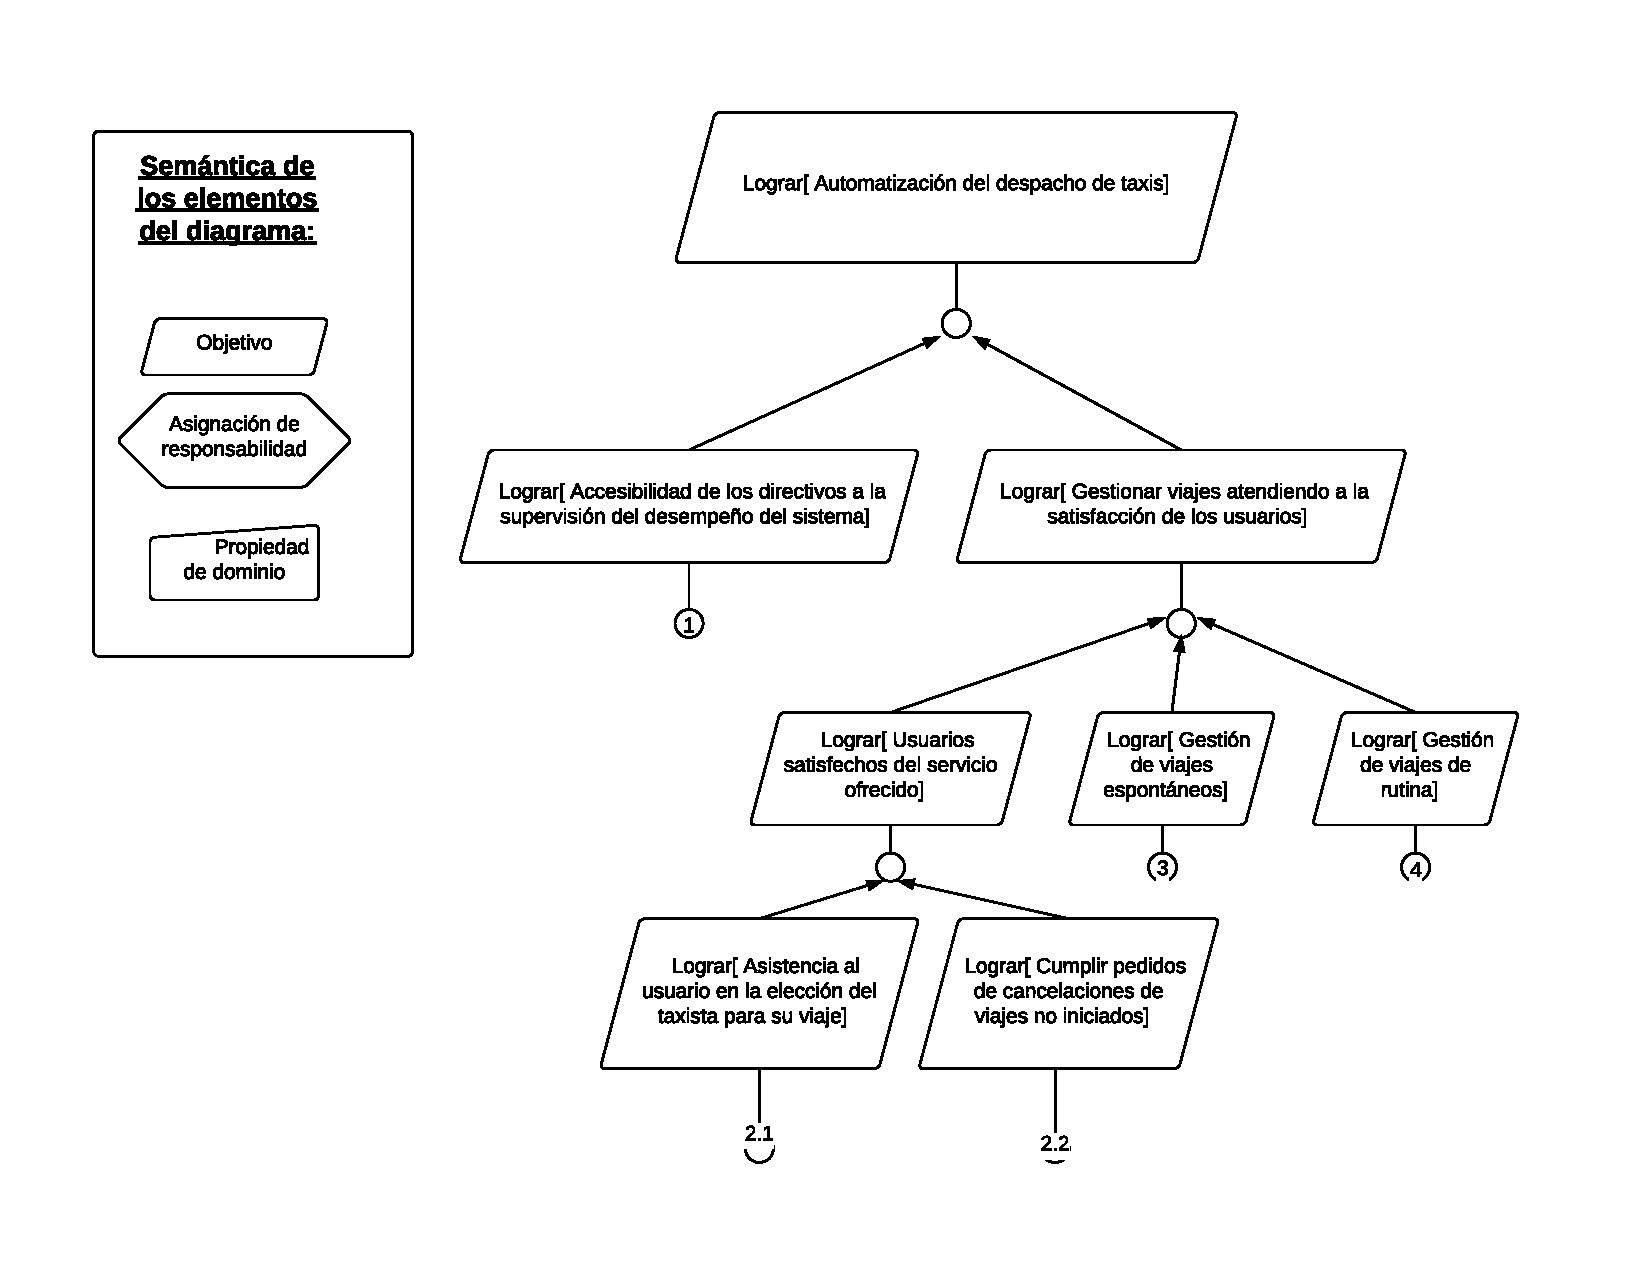
\includepdf[pages={1}, pagecommand=\subsection{Automatización del despacho de taxis}, scale=1]{Objetivos-nuevo-modificado}
\includepdf[pages={2}, pagecommand=\subsection{Accesibilidad de los directivos a la supervisión de TecnoTaxi}, scale=1]{Objetivos-nuevo-modificado}
\includepdf[pages={3}, pagecommand=\subsection{Usuarios satisfechos del servicio ofrecido - Elección taxista}, scale=1]{Objetivos-nuevo-modificado}
\includepdf[pages={4}, pagecommand=\subsection{Gestión de viajes espontáneos}, scale=1]{Objetivos-nuevo-modificado}
\includepdf[pages={5}, pagecommand=\subsection{Gestión de viajes espontáneos - Pago del Viaje}, scale=1]{Objetivos-nuevo-modificado}
\includepdf[pages={6}, pagecommand=\subsection{Gestión de viajes de rutina}, scale=1]{Objetivos-nuevo-modificado}
\includepdf[pages={7}, pagecommand=\subsection{Gestión de viajes de rutina - Pago anticipado}, scale=1]{Objetivos-nuevo-modificado}
\includepdf[pages={8}, pagecommand=\subsection{Gestión de viajes de rutina - Pago en efectivo}, scale=1]{Objetivos-nuevo-modificado}
\includepdf[pages={9}, pagecommand=\subsection{Usuarios satisfechos del servicio ofrecido - Cancelación de viaje}, scale=1]{Objetivos-nuevo-modificado}
\includepdf[pages={10}, pagecommand=\subsection{Usuarios satisfechos del servicio ofrecido - Cancelación de Viaje - Aviso al taxista}, scale=1]{Objetivos-nuevo-modificado}

\section{Observaciones}
\begin{itemize}

\item En esta versión final del diagrama de objetivos, el requerimiento 3 enunciado en el TP2, se encuentra representado en el \textbf{\ref{req:R15}}.
\item El \textbf{\ref{req:R4}} atiende al planteo, originalmente plasmado en el enunciado, de que \emph{el taxista no reciba constantes mensajes de radio que lo incomodan}.
\item El \textbf{\ref{req:R21}} se asigna conjuntamente a TecnoTaxi y a la operadora, dado que será la operadora la que tomará la solicitud del viaje por teléfono, accediendo ella a las opciones que ofrece TecnoTaxi en nombre del pasajero.
\item El \textbf{\ref{req:R27}} es importante para continuar con el proceso de elección de un taxista para efectivizar el viaje. 
\item En el caso de los viajes de rutina, es decir, con reserva, el taxista no será el encargado de indicar el importe del viaje de la manera tradicional -como lo hace en el pago en efectivo de un viajhe espontáneo- sino que TecnoTaxi se lo informará (\textbf{\ref{req:R35}}).
\item En lo que respecta a la satisfacción del deseo del usuario de poder \emph{conocer la ubicación del taxi que encargó para tener la oportunidad de cancerlarlo }(tal cual se manifestara en el enunciado original de este trabajo), tenemos el \textbf{\ref{req:R37}}
\item También al satisfacer el deseo del usuario de cancelar un viaje, aparece la necesidad de notificar al taxista inmediatamente. Consideramos aquí un o-refinamiento: Se evaluó la alternativa de manejar la comunicación solamente por SMS. A pesar de ser más barata en costo, en el trabajo resultante optamos por la versión descripta del sistema de radio para las contingencias, y el resto por la computadora con internet embebida en el taxi. Se priorizó la mayor confiabilidad en la recepción de la información, y la mayor facilidad de uso.

\end{itemize}
